\chapter{Discussion}
\label{Discussion}
This section presents an analysis and discussion of the results. 

\section{Graph Behavior}
The behaviors shown in \Cref{sec:results:graph_behavior}'s subsections and the graphs shown in \Cref{sec:apendixF:graph_behavior_with_IVA} represent typical trends observed when varying the parameter values. 
The graph behavior should be interpreted in conjunction with the local $S1$ sensitivities from \Cref{sec:Sobol_sensitivity_analysis_results} to gain a better understanding of how sensitive the output is to specific parameters and the potential impact of variations in these parameters.

A researcher would examine the growth curve and conclude by visually analyzing the curves and reasoning through the ODE model to explain the behavior. 
They can further supplement this analysis with a Sobol analysis to quantify the significance of the change and compare the importance of a parameter with that of other parameters. 
By analyzing the $S$ and $S1$ values, they can also determine if the parameter acts mostly independent of other parameters or work closely with other parameters. 
If the parameter interacts with other parameters, then those parameters need to be changed to notice a significant difference in the output. 

\section{Realistic Growth Curves}
As the complexity of the network increases, biologically accurate curves become more complicated. 
There isn't just an exponential and death cycle anymore, but rather a combination of multiple phases for an individual species in a complex community. 
This can be seen in real complex communities where there are multiple phases happening at the same time. 

In a $1\times 1\times 1$ system, like that in \Cref{fig:created:a_good_curve}, there is a clear exponential growth, peak, and death cycle for the bacteria. 
The phages experience a delay in growth but also exhibit exponential growth. 
These behaviors can disappear as the community size grows to a $p\times b\times r$ system. 
\Cref{fig:created:large_graph_network_output} shows how these behaviors disappear. 
Some, but not every phage or bacteria in \Cref{fig:created:large_graph_network_output} exhibits a clear growth and death cycle. 
Bacteria face increased competition for resources, and phages face increased competition for bacteria. 
This increased competition decreases the pool of available resources for the bacteria and phages to grow. 
There is an external threat known as the washout, which cancels out bacterial and phage growth. If the growth is not fast enough, it can even be eliminated. 

There are only two interactions that occur in a $1\times1\times1$ system. 
With a $p\times b\times r$ system, there are at most $p\cdot b + b\cdot r$ interactions that can occur. 
Any number of phages can interact with any number of bacteria, and any number of bacteria can interact with any number of resources, each with its unique parameter values. 
These varying rates will influence the system's dynamics, making it difficult to determine which event caused what due to the increased complexity of the network. 
With so many individual events co-occurring, it becomes more challenging to identify the cause of the event and how its action will propagate through the network. 

There are ways to circumvent this issue. 
Simulations offer researchers the ability to experiment with systems that might not be feasible otherwise. 
Knocking out specific nodes or edges and rerunning the simulation would enable the researcher to observe how the removal of the knocked-out node or edge affected the simulation. 
The knocked-out node or edge will no longer contribute to the simulation, resulting in an impact on the population count. 
The larger the difference, the more critical that node or edge was in the simulation. 

\subsection{Knockout}
\Cref{fig:created:large_graph_network_output} (original plot) and \Cref{fig:created:large_graph_network_output_knockout_B14_P2} (knocked out plot) show the difference that knockout has on the output of the graphs. 
In The original plot, there was more competition for the resources, and more phage populations infecting the bacteria. 
The bacteria died out earlier, so less resources were consumed. 
The washin kept on adding more resources to the system which causes the resource concentration to increase. 
$P_2$ and $B_{14}$ were knocked out of the network, using \Cref{fig:ss:example_large_network} as the base network and the parameter values were sampled in the ranges found in \Cref{tab:appendixE:Sobol_analysis_values}. 
In the knocked-out graph, more bacteria were able to survive, and in total, there were more bacteria in the system, as evidenced by the bacteria sum. 
There are also fewer infected bacteria. 
With the phages, there is less of a noticeable difference in behavior, but in \Cref{fig:created:large_graph_network_output}, $P_{18}$, pink, suddenly increases in concentration at $t=10$ until the end of the simulation, while this doesn't happen in \Cref{fig:created:large_graph_network_output_hidden_B14_P2}. 
$P_{18}$ infects $B_{14}$ (as well as $B_13$), so by removing $B_{14}$, $P_{18}$ was negatively affected, and explains why $P_{18}$ couldn't grow. 

By removing $P_2$ and $B_{14}$, it was demonstrated how the resource, bacterial, and phage dynamics were permanently altered. 
\Cref{fig:created:large_graph_network_output_knockout_B14_P2} showed how knockouts have a lasting impact on the dynamics of the system, changing which phages and bacteria survive. 

\begin{figure}
    \centering
    \begin{subfigure}{1\linewidth}
        \centering
        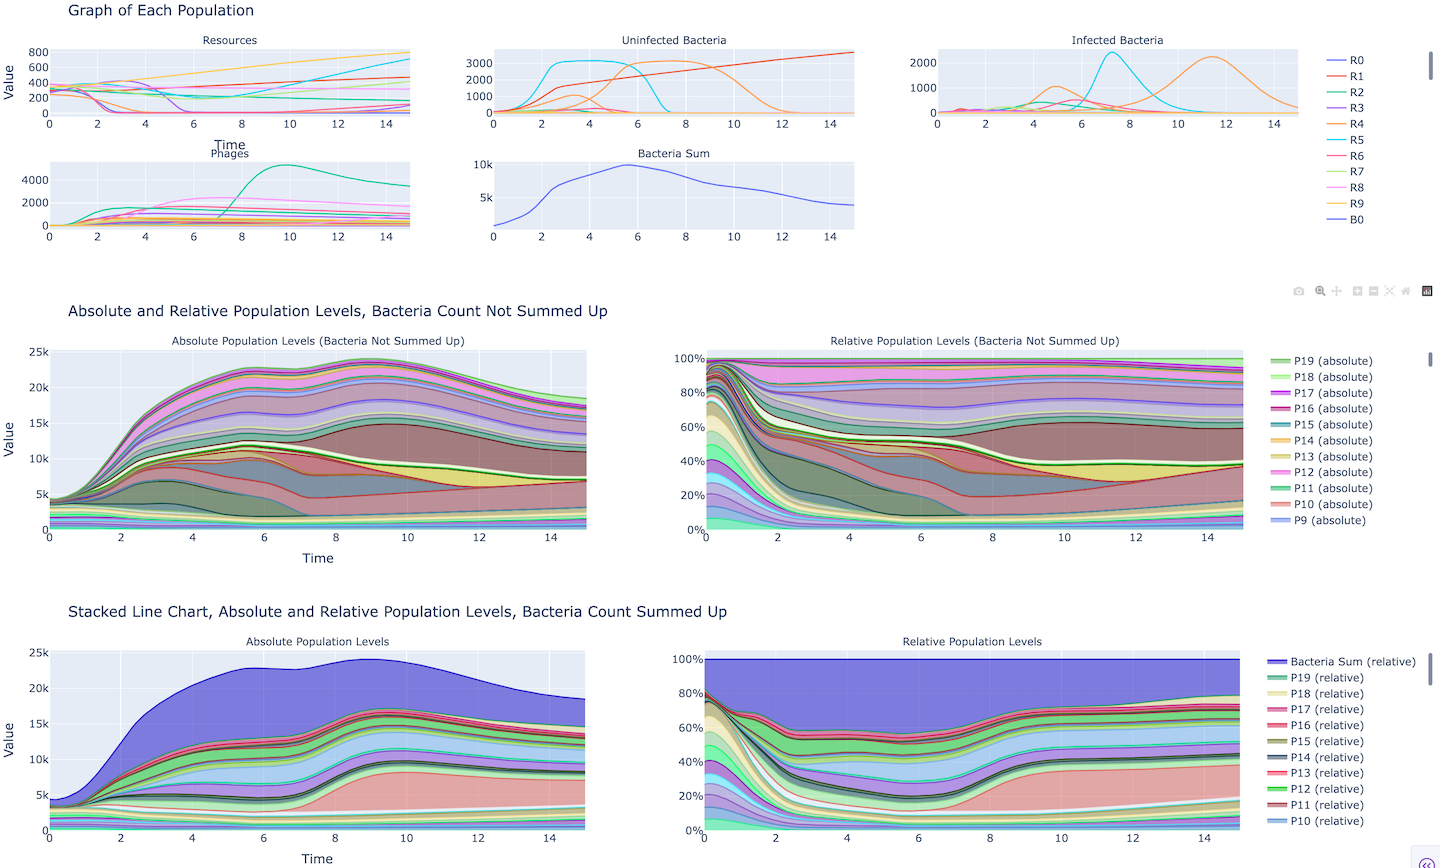
\includegraphics[width=\linewidth]{Plots/Created/large_graph_network_output.png}
        \caption{
            The output graph for the default parameter values for a $20\times 20 \times 10$ network. 
            Parameter values were randomly chosen in the interval given by \Cref{tab:appendixE:Sobol_analysis_values}. 
            The washin rate kept on adding more resources to the system. 
        }
        \label{fig:created:large_graph_network_output}
    \end{subfigure}
    \hfill
    \begin{subfigure}{1\linewidth}
        \centering
        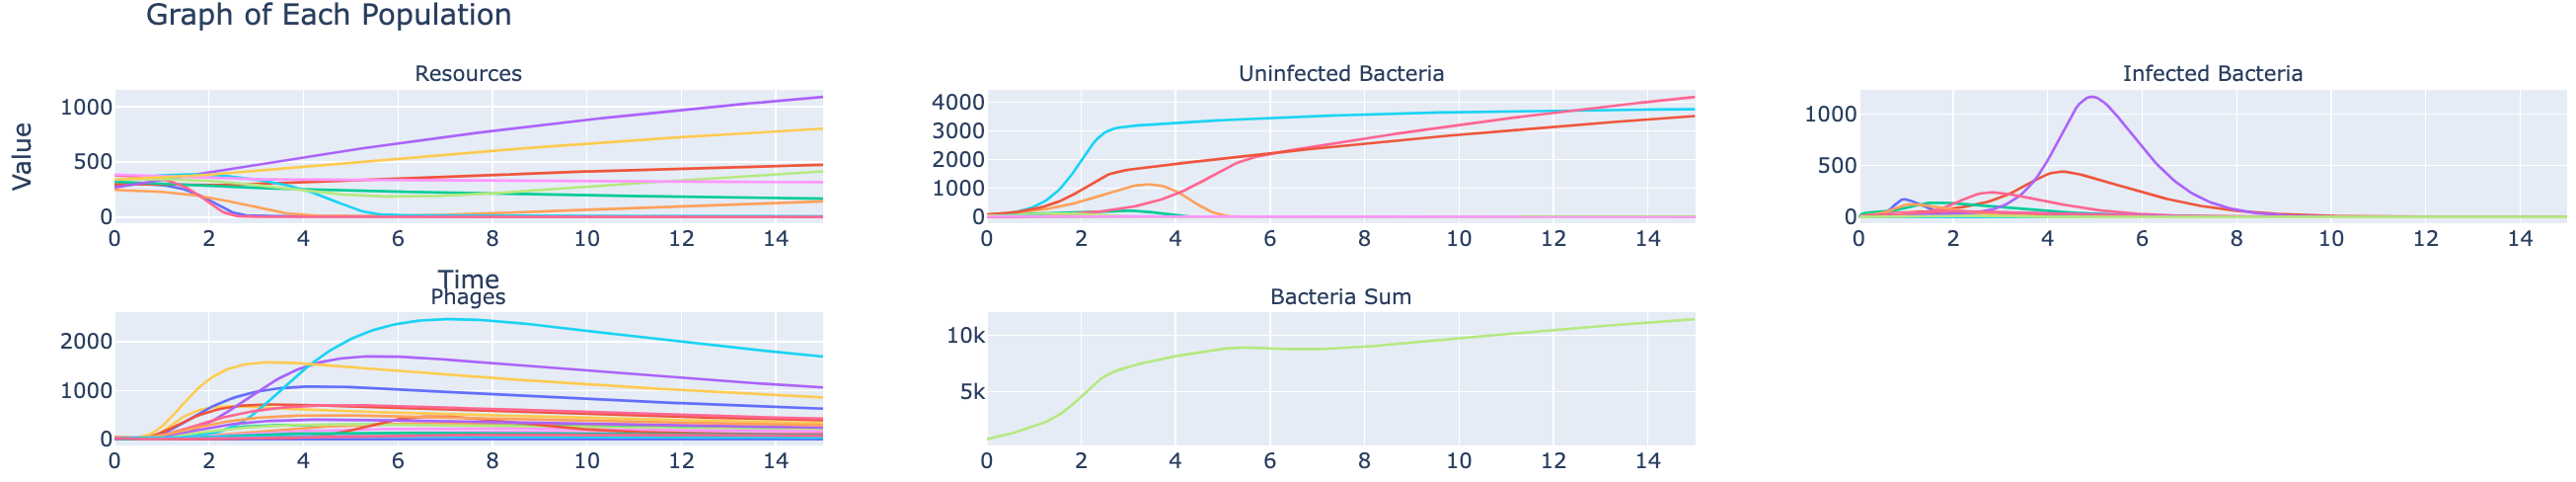
\includegraphics[width=\linewidth]{Plots/Created/large_graph_network_output_knockout_B14_P2.png}
        \caption{
            The large $20\times 20\times 10$ network, with phage $P_2$ and bacteria $B_{14}$ knocked out from the system.
        }
        \label{fig:created:large_graph_network_output_knockout_B14_P2}
    \end{subfigure}
    \caption{
        Comparing the effect of knocking $P_2$ and $B_{14}$ out from the system. 
        Figure a) has $P_2$ and $B_{14}$ hidden from the system, while Figure b) has the phage and bacteria knocked out from the system. 
        The most important phage and bacteria, as indicated by the growth of bacteria, were knocked out. 
        \Cref{fig:ss:example_large_network} is used as the reference network model. 
        The colors between a) and b) cannot be directly compared, as the color is not mapped to a specific phage or bacterium. 
    }
\end{figure}

\section{Sobol Sensitivity}
A researcher may have an intuitive understanding of how a model works but may be uncertain about the significance of the model's parameters to its results.  
A researcher can use Sobol to quantify the importance of a change in parameter value in the context of the simulation results. 
By testing and measuring hundreds of simulation inputs and outputs, Sobol understands how changing a parameter's value influences its output. 
By identifying the critical parameters, a researcher could use that to their benefit in their research. 
Researchers can prioritize adjusting the most influential parameters in their simulations or consider engineering phages and bacteria to achieve the desired parameter values.

This section provides a more in-depth discussion of the Sobol results from \Cref{sec:Sobol_sensitivity_analysis_results}. 

\subsection{Resources}
Every parameter affects how the bacterial and phage populations grow, which in turn influences the consumption rate of resources and ultimately determines the final resource value. 
Greater resource consumption leads to a lower final resource level.
As most resources are typically consumed by the end of the simulation, the final resource value will be 0. 
However, some parameters, such as $\tau$ and $\beta$, have a more significant influence on the depletion rate of resources than others. 
Of all parameters, $\tau$ has the most significant influence on the final resource value. 
$\tau$ determines how fast the bacteria will go through the infection process. 
The longer it takes (i.e., the bigger the value of $\tau$ is), the longer it takes for the phage population to grow, allowing more bacteria to grow and consume resources. 
For smaller $\tau$ values, the phages can quickly grow, infect, and kill the bacteria. 
For large $\tau$ values the bacteria will die early and not consume any resources anymore. 
There are some combinations of parameters that, when chosen, will result in not all the resources being used up. 
For example, with \Cref{tab:appendixE:a_good_curve_2}, if $r = 0.2$, not all the resources have been used up. 
$r$ defines the probability of a phage infecting a resource. 
$r$ being so high will cause the phages to initially infect many bacteria. 
However, due to the high infection rate, most bacteria are immediately infected, preventing the population growth, and die out quickly. 
Therefore, the final resource value will still be relatively high because the bacteria did not have the opportunity to consume the resources. 

\subsection{Phages}
$r$, the adsorption rate of phages to bacteria, is the probability of a successful infection. 
The smaller the value, the less likely it is to result in a successful infection. 
With a larger $r$ value, the likelihood of an infection occurring increases. 
$r$ is the most important value for determining the final phage value. 
$\beta$ influences the final phage population, as the infected bacterium will release $\beta$ phages into the system. 
The larger $\beta$ is, the more phages can be created. 
The more phages that are created for every lysed bacterium, the more phages are available in the system to infect the bacteria. 

The barplot values for the peak value of phages using the 95\% rule match the final value plot for the phages. 
This makes sense as there is no removal of phages from the system, so any phages created by the lysis that are heavily influenced by $r$ and $\beta$ will stay in the system. 
As the population continues to increase, the final and peak values will occur near one another (due to the 95\% rule) and are closely associated with each other.

$\tau$, the latent infection period, emerges as the most critical parameter, setting the peak time for the phage population. 
The $\tau$ parameter determines the rate at which an infected bacterium progresses through the infection process. 
Decreasing tau increases the speed of lysis, allowing more phages to be produced faster. 
More phages earlier in the system's will allow more infections to occur, thereby decreasing the pool of available bacteria. 
This, in turn, will increase the phage population more rapidly than other parameters, resulting in the phages reaching their peak population faster.
$r$ and $\beta$ (the burst size) have similar effects, but they affect the final and peak phage population rather than the amount of time it takes to reach the peak value. 
By changing $\beta$ and $r$, more phages or fewer phages are released, rather than specifically speeding up a process that $\tau$ does. 
Holding $\beta$ constant, increasing $r$ will increase more phages released, but fewer phages will be made in total because the phages will infect the bacteria faster. 
This will help phages grow in population faster; however, the bottleneck is how quickly phages can be created, which is determined by $\tau$. 
Changing $r$ and $\beta$ won't have as significant of an impact on the time to peak as $\tau$ does, as $\tau$ shortens the infection period, literally decreasing the time until new phages are created and directly affecting how fast phages can be produced. 

\subsection{Total Bacteria}
Resources, $\tau$, $e$ (the resource consumption probability), and $\beta$ all play a critical role in the final population value of bacteria. 
That being said, 
More resources allow bacteria to grow for a more extended period, enabling the creation of more bacteria. 
$\beta$ plays a crucial role in determining the final bacterial population, whereas $r$ has no significant impact on the final bacterial population. 
$e$ determines the resource consumption rate. 
The larger $e$ is, the faster the resource's depletion rate. 
So, by lowering $e$, more bacteria will be created, and the time at which the bacteria peak occurs later. 

The total bacteria peak population is much more sensitive to the different parameter values. 
The bacteria act as a link between the phages and resources. 
Any changes in the resource consumption rate or initial condition will affect the bacteria population. 
Likewise, any change in phage adsorption rate will affect the bacteria growth, which in turn will affect the resource consumption rate. 
The bacteria can dampen the effect of specific parameters. 
For example, the initial resource value affects the final resource value. 
The initial resource value partially affects the final bacteria value, but it doesn't affect the phages. 
The parameters lose strength as they propagate through the system. 
Since the bacteria exist between the phages and resources, they are exposed to various parameters that ultimately influence the peak value. 
Many of these parameters interact with one another; hence, $ST > S1$ is true for many of the inputs. 

Similar to the peak value, bacteria interact with multiple parameters that influence other parameters. 
The peak value, on the other hand, has no limit on the peak value, with a peak value occurring anywhere between 0 and $\infty$. 
The time of peak value depends on higher-order interactions for $e$ and $K$ as the bacteria grow at the Monod equation rate. Therefore, $e$ and $K$ (the Monod constant) are only important when combined with changing other parameter values. 
To find these critical parameters, the third, fourth, fifth, and subsequent orders will need to be calculated to determine which pairs of parameters interact with $e$ and/or $K$ and have the most significant impact on variance in the output. 

\section{Initial Value Analysis}
\citet{mullaExtremeDiversityPhage2024} identify two key processes that dictate the growth of bacteria. 
Phages adsorb to bacteria, and bacteria lyse bacteria after a time delay. 
The authors investigate which of the two steps limits the infection cycle rate. 
They find that there is an analytical solution to the time of peak value in an adsorption limited regime for the bacteria population is $t_{\text{col}} = \frac{1}{r_{\text{bac}}} \log\left(1 + \frac{r_{\text{bac}}}{r_{\text{pha}}b_0} \log\left(\frac{p_{\infty}}{p_0}\right)\right)$, where $p_0$ is the initial phage value, $p_\infty$ is the final phage value, $r_{\text{pha}} = n_{\text{burst}} k_{\text{absorb}}, n_{\text{burst}}$ is the burst size, $k_{\text{absorb}}$ is the absorption rate, $r_{\text{bac}}$ is the bacteria growth rate, $b_0$ is the initial bacteria concentration. 
They demonstrate that the time of peak value is primarily limited by phage-bacteria adsorption and that the adsorption rate depends on the bacterial concentration, whereas the burst rate does not. 
The region is adsorption limited when $k_{absorb}b(t) \ll k_{burst}$. 
If the system is burst limited, the time of collapse can be calculated as follows: $t_{\text{col}} = \frac{\log\left(\frac{r_{\text{bac}}}{k_{\text{burst}}}\left(\frac{1}{n_{\text{burst}}} + \frac{1}{\text{MOI}_0} - \frac{r_{\text{bac}}}{k_{\text{burst}}}\right)\right)}{k_{\text{burst}}n_{\text{burst}} - r_{\text{bac}}}$ \cite{mullaExtremeDiversityPhage2024}. 

The behavior between \Cref{fig:created:initial_value_analysis_UB_50_500_a_good_plot_2} and \Cref{fig:created:initial_value_analysis_UB_50_500_a_good_plot} should be similar. However, the change in parameter values altered the simulation to introduce a region in behavior change. 
It would be expected that for 100 initial uninfected bacteria and fewer, the bacteria sum peak time would follow the linear regression line; however, at around 100 uninfected bacteria, the peak curve deviates from the linear expression. 

Between 100 and 500 uninfected bacteria, the system is adsorption limited.
The curve follows what was proposed by \citet{mullaExtremeDiversityPhage2024} 
The adsorption of phages to bacteria depends on the initial bacterial concentration \cite{mullaExtremeDiversityPhage2024}. 
For larger uninfected bacteria populations, the infection process speeds up as a larger proportion of bacteria can be infected $r\cdot U\cdot P$, where $r$ is the successful phage-bacteria adsorption rate. 

The bacteria can grow without immediate pressure from the phages. 
For small initial resource concentrations and initial bacterial populations, the resources will quickly become depleted. 
This severely limits the bacteria's ability to grow and artificially caps the population. 

The system is latency-limited between 25 and 100 uninfected bacteria. 
As the initial bacteria decreases, we transition out of the $k_{\text{absorb}}b \ll k_{\text{burst}}$ equality as identified as a condition for the adsorption-limited regime. 
The phage-to-bacteria ratio increases, allowing them to infect the bacteria more quickly. 
Therefore, the time to phage peak also decreases as the initial number of uninfected bacteria decreases. 

As the uninfected bacteria decreases from 25 to 1, it takes longer for the bacteria to grow and reach their peak population count. 
At these initial bacterial concentration levels, there are sufficient resources to sustain the bacteria throughout the entire simulation. 
For uninfected bacteria with fewer than 25, the system enters a new type of restriction, where it experiences a delay in infection due to low encounter rates. 

The transition rate from uninfected bacteria $U$ to the first infected stage $I_1$ is proportional to $U\cdot P$. 
Fewer bacteria are initially infected when the starting number of bacteria is low. 
If the phages can't infect the bacteria, the later infection stages are delayed due to the slow infection process. 
There could be a threshold for phage to uninfected bacteria where a specific dilution rate will significantly affect the peak time. 
This value could be approximately $\frac{\text{initial phage}}{\text{initial bacteria}} = \frac{10}{25} = 0.4$, as the system transitions from a latency-limited to a new limited regime around 25 uninfected bacteria. 
The bacteria have a more extended period to grow, as there is a low infection rate and ample resources to consume. 
This means that it takes longer for the bacteria to grow, as noticed by the increase in peak time relative to larger initial uninfected bacteria populations. 
As the bacteria population drives the phage population, an increase in bacteria time of peak causes an increase in phage time of peak. 

\section{Phage Proliferation}
If the adsorption rate $r$ is too large and/or burst size $\beta$ is too small, the phages will disappear when washout is included. 
Without phage washout, the phages will eventually take over the bacteria, no matter the initial conditions. 

Ensuring that there are initially sufficient phages in an experiment, as well as an appropriate $r$ and $\beta$ value to prevent them from disappearing from the system is crucial. 
Given the context of the Golding model, the easiest parameters that a researcher can control are the initial concentrations of phage, bacteria, and resources. 
Assuming an appropriate $r$ and $\beta$ value has been chosen, understanding how changing the initial phage, uninfected bacteria, and resource values will influence if phages can proliferate is essential. 
If there aren't enough initial resources or bacteria, the resources will be depleted by the bacteria, and the remaining bacteria will consume the remaining resources, resulting in limited bacterial growth. 
Limited bacterial growth means limited phage growth and the phages will be washed away. 

\subsection{Phase Portrait}
There is a non-linear trade-off between initial resources and initial phages when a washout is included. 
The washout non-linearly affects whether the phages proliferate or not. 
The larger the washout value, the more difficult it is for phages and bacteria to proliferate. 
The bacteria couple the phage populations to resources, so changes in initial resource concentration will affect the final phage value. 
Increasing the initial resource concentration leads to an increase in bacteria while decreasing it results in fewer bacteria.
More bacteria ultimately produce more phages, while fewer bacteria ultimately result in fewer phages.
While Sobol with washin and washout, \Cref{fig:created:Sobol_peak}, showed that the final value for phages due to changes in initial resource input values is limited (sensitivity $\approx 0.1$), it still has an impact. 

For low initial resource concentration values, those below $10$, the Monod curve is below the half-growth rate constant (where the growth rate $v$ is 1 and $K$ is 10). 
The lack of resources restricts the bacteria's growth, and the bacteria will grow below their maximum growth rate as they are being limited by the available resources. 
As the resource concentration increases towards $K=10$, the bacteria can grow faster. 
Since $K$ is small, a slight change in $R$ causes a relatively large change in the Monod rate. 

At around the minimum in the phage proliferation boundary, the behavior changes. 
As $R$ increases from $K$, the bacteria are no longer significantly limited by the nutrient concentration and can grow faster.
However, as $R$ increases beyond $K$, each additional unit of $R$ results in a diminishing rise in the Monod rate, which asymptotically approaches its maximum growth rate $v$. 

Phage proliferation becomes a race against time under external pressure. 
The phages will not proliferate if the phage growth rate is not fast enough to overcome the washout removal rate initially or if the infected bacteria are washed out before they lyse. 

\subsection{3D Plot}
It isn't easy to see inside the matrix, but using the color on the outside can give some insights into the behavior happening inside the matrix. 
The behavior inside the matrix is uniform with the behavior exhibited on the outside of the matrix. 
Even with the added bacteria, the phage proliferation boundary remains heavily dependent on the initial phages and initial resources rather than on the bacteria. 

\subsection{Ecology}
With the competitive exclusion principle in ecology, there should be at most 10 surviving bacteria in \Cref{fig:created:survivability} \cite{hardinCompetitiveExclusionPrinciple1960}. 
Two or more species competing for the same resources can not coexist indefinitely. 
The $\text{R}^{*}$ resource-ratio hypothesis states that a species must be the best at consuming resources to persist. 
Populations that need a high resource availability will need to either adapt or die out when competing against a population with a low resource consumption. 
A species can only survive in steady state at the lowest level of limiting resource $R^{*}$, excludes all other species \cite{juRuleEnergyFlux2009}. 
The species with the lowest $\text{R}^{*}$ for a shared limiting resource will out compete the others and dominate in the long term.
The growth rate of a species is proportional to the resources consumed with an energy factor minus a maintenance and death rate. 
The bigger the resource overlap between competing bacteria, the smaller the realm of co-existence \cite{vandenbergEcologicalModellingApproaches2022}. 
Populations that are slow at consuming resources reproduce at a slower rate and thus will eventually die out. 
For a species that consumes multiple resources, the growth of the species is defined by the largest $\text{R}^{*}$, as that resource is limiting the growth. 

The Zero Net Growth Isoclines (ZNGI) graph shows how a species transitions between being limited by $R_1$ to being limited by $R_2$. 
The isocline defines the optimal supply ratio at which a bacteria transitions from being limited by $R_1$ to being limited by $R_2$. 
The isocline represents where cell growth = cell death. 
With multiple isoclines, with each isocline representing a bacteria strain, you can tell which strain will outcompete and proliferate, and under which initial resource concentrations coexistence can occur \cite{smithEffectsResourceSupplies2002}.